\chapter{Конструкторская часть}
В данном разделе будут приведены схемы алгоритмов нахождения расстояния Левенштейна и
Дамерау-левенштейна.

\section{Схемы алгоритмов}

Алгоритмы на вход получают строчки $S_1$ и $S_2$, а на выходе возвращают целое число,
которое показывает расстояние.

На рисунках \ref{fig:images-rec-lev} --- \ref{fig:images-ddyn-lev}
представлены схемы алгоритмов нахождения расстояния Левенштейна и Дамерау-Левенштейна.

\begin{figure}[h]
    \centering
    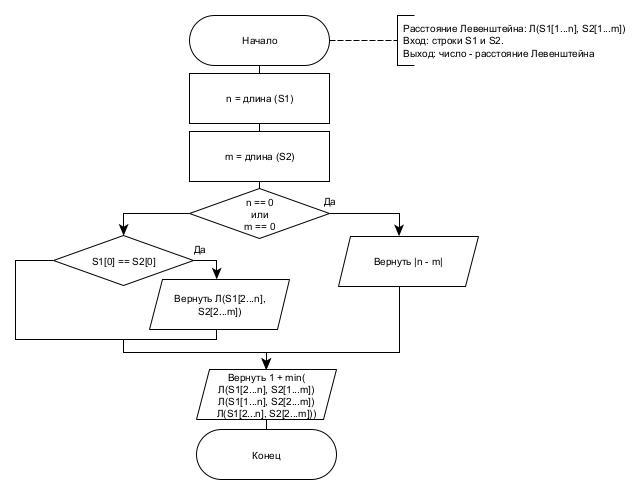
\includegraphics[width=0.8\textwidth]{images/lev_rec.jpg}
    \caption{Схема рекурсивного алгоритма расстояния Левенштейна}
    \label{fig:images-rec-lev}
\end{figure}

\clearpage

\begin{figure}[h]
    \centering
    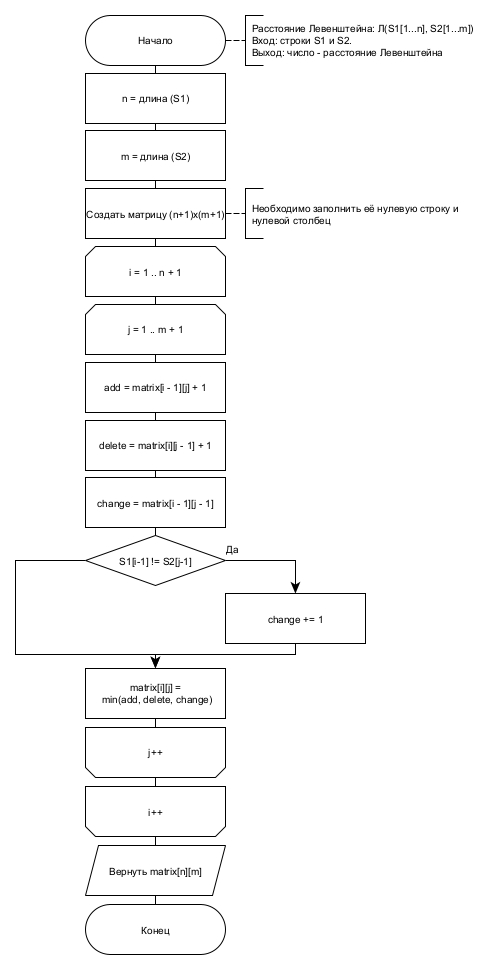
\includegraphics[width=0.6\textwidth]{images/lev_dyn.jpg}
    \caption{Схема динамического алгоритма расстояния Левенштейна}
    \label{fig:images-dyn-lev}
\end{figure}

\clearpage

\begin{figure}[h]
    \centering
    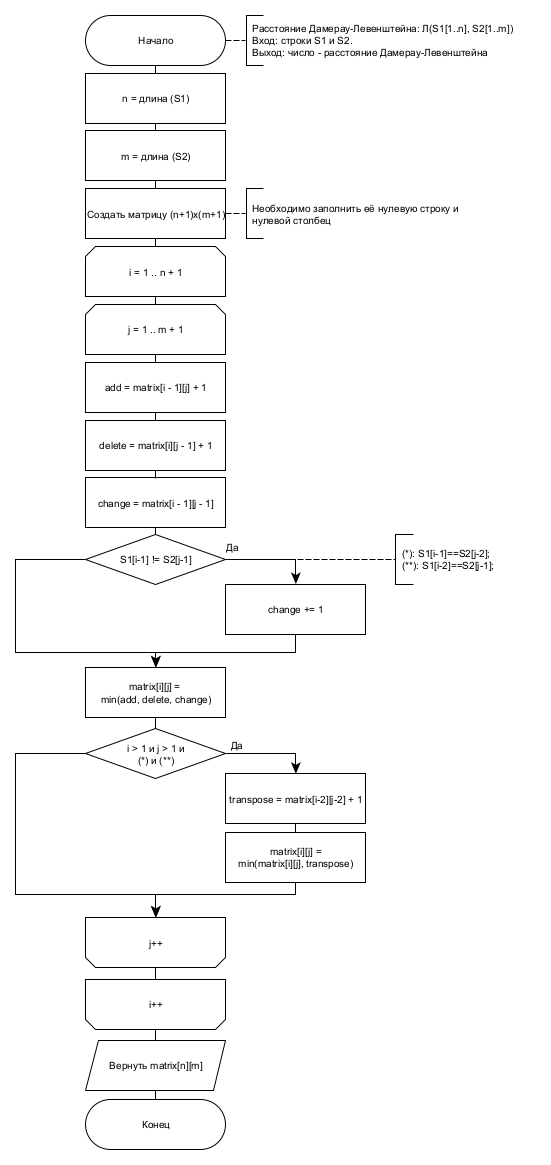
\includegraphics[width=0.6\textwidth]{images/d_lev_dyn.jpg}
    \caption{Схема динамического алгоритма расстояния Дамерау-Левенштейна}
    \label{fig:images-ddyn-lev}
\end{figure}

\clearpage

\paragraph*{ВЫВОД} ${}$ \newline
В данном разделе были представлены схемы алгоритмов нахождения расстояния Левенштейна и
Дамерау-Левенштейна.


\clearpage
